%Version 2.1 April 2023
% See section 11 of the User Manual for version history
%
%%%%%%%%%%%%%%%%%%%%%%%%%%%%%%%%%%%%%%%%%%%%%%%%%%%%%%%%%%%%%%%%%%%%%%
%%                                                                 %%
%% Please do not use \input{...} to include other tex files.       %%
%% Submit your LaTeX manuscript as one .tex document.              %%
%%                                                                 %%
%% All additional figures and files should be attached             %%
%% separately and not embedded in the \TeX\ document itself.       %%
%%                                                                 %%
%%%%%%%%%%%%%%%%%%%%%%%%%%%%%%%%%%%%%%%%%%%%%%%%%%%%%%%%%%%%%%%%%%%%%

\documentclass[sn-basic,pdflatex]{sn-jnl}

%%%% Standard Packages
%%<additional latex packages if required can be included here>

\usepackage{graphicx}%
\usepackage{multirow}%
\usepackage{amsmath,amssymb,amsfonts}%
\usepackage{amsthm}%
\usepackage{mathrsfs}%
\usepackage[title]{appendix}%
\usepackage{xcolor}%
\usepackage{textcomp}%
\usepackage{manyfoot}%
\usepackage{booktabs}%
\usepackage{algorithm}%
\usepackage{algorithmicx}%
\usepackage{algpseudocode}%
\usepackage{listings}%
%%%%

%%%%%=============================================================================%%%%
%%%%  Remarks: This template is provided to aid authors with the preparation
%%%%  of original research articles intended for submission to journals published
%%%%  by Springer Nature. The guidance has been prepared in partnership with
%%%%  production teams to conform to Springer Nature technical requirements.
%%%%  Editorial and presentation requirements differ among journal portfolios and
%%%%  research disciplines. You may find sections in this template are irrelevant
%%%%  to your work and are empowered to omit any such section if allowed by the
%%%%  journal you intend to submit to. The submission guidelines and policies
%%%%  of the journal take precedence. A detailed User Manual is available in the
%%%%  template package for technical guidance.
%%%%%=============================================================================%%%%

%% Per the spinger doc, new theorem styles can be included using built in style, 
%% but it seems the don't work so commented below
%\theoremstyle{thmstyleone}%
\usepackage{booktabs}
\newtheorem{theorem}{Theorem}%  meant for continuous numbers
%%\newtheorem{theorem}{Theorem}[section]% meant for sectionwise numbers
%% optional argument [theorem] produces theorem numbering sequence instead of independent numbers for Proposition
\newtheorem{proposition}[theorem]{Proposition}%
%%\newtheorem{proposition}{Proposition}% to get separate numbers for theorem and proposition etc.

%% \theoremstyle{thmstyletwo}%
\theoremstyle{remark}
\newtheorem{example}{Example}%
\newtheorem{remark}{Remark}%

%% \theoremstyle{thmstylethree}%
\theoremstyle{definition}
\newtheorem{definition}{Definition}%

\usepackage{booktabs}
\usepackage{longtable}
\usepackage{array}
\usepackage{multirow}
\usepackage{wrapfig}
\usepackage{float}
\usepackage{colortbl}
\usepackage{pdflscape}
\usepackage{tabu}
\usepackage{threeparttable}
\usepackage{threeparttablex}
\usepackage[normalem]{ulem}
\usepackage{makecell}
\usepackage{xcolor}


\raggedbottom




% tightlist command for lists without linebreak
\providecommand{\tightlist}{%
  \setlength{\itemsep}{0pt}\setlength{\parskip}{0pt}}





\begin{document}


\title[Article Title runing]{Data Augmentation for Machine Learning}

%%=============================================================%%
%% Prefix	-> \pfx{Dr}
%% GivenName	-> \fnm{Joergen W.}
%% Particle	-> \spfx{van der} -> surname prefix
%% FamilyName	-> \sur{Ploeg}
%% Suffix	-> \sfx{IV}
%% NatureName	-> \tanm{Poet Laureate} -> Title after name
%% Degrees	-> \dgr{MSc, PhD}
%% \author*[1,2]{\pfx{Dr} \fnm{Joergen W.} \spfx{van der} \sur{Ploeg} \sfx{IV} \tanm{Poet Laureate}
%%                 \dgr{MSc, PhD}}\email{iauthor@gmail.com}
%%=============================================================%%

\author*[1]{\fnm{Ae
Kyong} \sur{Jung} }\email{\href{mailto:aekyong-jung@uiowa.edu}{\nolinkurl{aekyong-jung@uiowa.edu}}}

\author[2]{\fnm{Second} \sur{Author} }



  \affil*[1]{\orgdiv{Department}, \orgname{Organization}, \orgaddress{\city{City}, \country{Country}, \postcode{100190}, \state{State}, \street{Street}}}
  \affil*[2]{\orgname{Other Organisation}}

\abstract{\textbf{Purpose}: The abstract serves both as a general
introduction to the topic and as a brief, non-technical summary of the
main results and their implications. The abstract must not include
subheadings (unless expressly permitted in the journal's Instructions to
Authors), equations or citations. As a guide the abstract should not
exceed 200 words. Most journals do not set a hard limit however authors
are advised to check the author instructions for the journal they are
submitting to.}

\keywords{data augmentation, SmoteR, Catalytic Prior}


\pacs[JEL Classification]{D8, H51}
\pacs[MSC Classification]{35A01, 65L10}

\maketitle

\begin{center}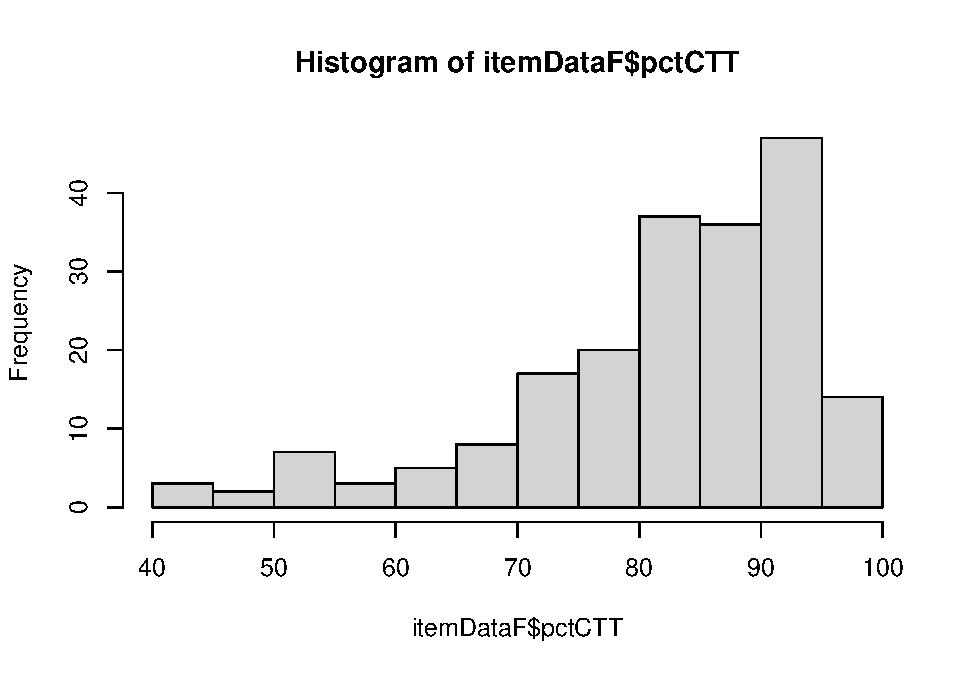
\includegraphics{Data-augmentation_files/figure-latex/plot_data_distribution-1} \end{center}

\begin{verbatim}
## $breaks
##  [1]  40  45  50  55  60  65  70  75  80  85  90  95 100
## 
## $counts
##  [1]  3  2  7  3  5  8 17 20 37 36 47 14
## 
## $density
##  [1] 0.003015075 0.002010050 0.007035176 0.003015075 0.005025126 0.008040201
##  [7] 0.017085427 0.020100503 0.037185930 0.036180905 0.047236181 0.014070352
## 
## $mids
##  [1] 42.5 47.5 52.5 57.5 62.5 67.5 72.5 77.5 82.5 87.5 92.5 97.5
## 
## $xname
## [1] "itemDataF$pctCTT"
## 
## $equidist
## [1] TRUE
## 
## attr(,"class")
## [1] "histogram"
\end{verbatim}

\begin{center}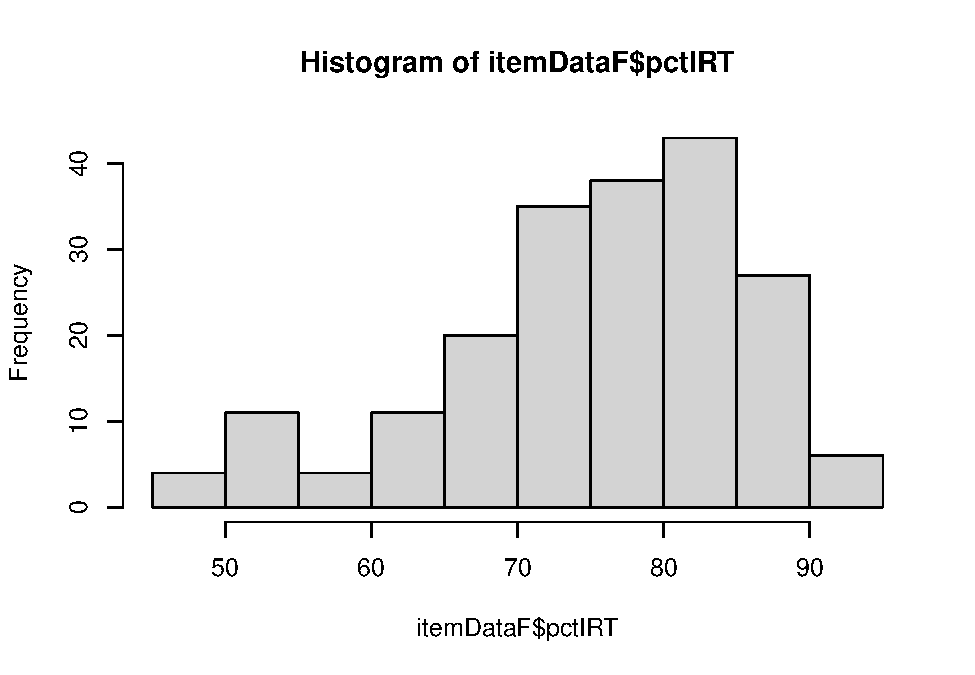
\includegraphics{Data-augmentation_files/figure-latex/plot_data_distribution-2} \end{center}

\begin{verbatim}
## $breaks
##  [1] 45 50 55 60 65 70 75 80 85 90 95
## 
## $counts
##  [1]  4 11  4 11 20 35 38 43 27  6
## 
## $density
##  [1] 0.004020101 0.011055276 0.004020101 0.011055276 0.020100503 0.035175879
##  [7] 0.038190955 0.043216080 0.027135678 0.006030151
## 
## $mids
##  [1] 47.5 52.5 57.5 62.5 67.5 72.5 77.5 82.5 87.5 92.5
## 
## $xname
## [1] "itemDataF$pctIRT"
## 
## $equidist
## [1] TRUE
## 
## attr(,"class")
## [1] "histogram"
\end{verbatim}

\section{Introduction}\label{sec1}

The objective of data augmentation is to improve the performance of
learning model prediction on the rare cases. If there are majority
class, the model learn the data focusing on the majority class, which
lead to lower the performance of predicting on rare cases.

The primary objective of data augmentation is to generate ``good''
synthetic data which are rare cases. In this context, ``good'' synthetic
data effectively capture the underlying relationship between predictor
and target variables within training set. The ultimate goal is to train
a model that can accurately predict target variables from the predictor
variable in an unseen test set. To achieve this, we explored several
data augmentation techniques designed to create well-connected
predictor-target pairs. The methods investigated include random
oversampling, Gaussian Noise, SMOTER, SMOTGN, Importance Sampling,
Multiple Imputation, and the use of a catalytic prior.

\section{Data Augmentation}\label{sec2}

\subsection{Random Oversampling}\label{subsec2-1}

Replicate original data including target variable and predictors within
the threshold.

\begin{figure}[H]

{\centering \includegraphics[width=0.8\linewidth]{../../Plot_pctCTT_random} 

}

\caption{Relevance function and threshold for CTT}\label{fig:plot_relevance_ctt}
\end{figure}
\begin{figure}[H]

{\centering \includegraphics[width=0.8\linewidth]{../../Plot_pctIRT_random} 

}

\caption{Relevance function and threshold for IRT}\label{fig:plot_relevance_irt}
\end{figure}

\subsection{Gaussian Noise}\label{subsec2-2}

Add an error sampled from Normal(0, perc) to a rare case. Perc is
derived from the median of distances with the other rare cases from the
rare value. It is applied to the predictors and target value.

\subsection{SMOTE R}\label{subsec2-3}

Conduct interpolation between one rare case and the other rare case. The
other rare case is randomly selected within the k-nearest neighbors
among the rare cases. Between the two rare cases, interpolation is
applied. This is applied to predictor and target variable.

\subsection{SMOGN}\label{subsec2-4}

This is combination of Smote R and Gaussian Noise. When the other rare
case is within the safe zone which is close than the median of the
distances derived from all the distance from the seed rare case. If the
other rare case is not within the safe zone, then it is neglected and
Gaussian Noise method is applied.

\subsection{Importance Sampling}\label{subsec2-5}

\subsection{Multiple Imputation (DA-MI)}\label{subsec2-6}

This three-step method creates a synthetic dataset that mimics the
statistical properties of original, sensitive data. This allows
researchers to replicate findings without compromising the privacy of
individuals. 1. Generating pseudo-observations (w) by applying a masking
model to the original data. This process intentionally adds statistical
noise or otherwise perturbs the confidential values, effectively
creating a masked version of the dataset that obscures the true,
sensitive information. 2.Next, fit a joint imputation model by
integrating two distinct parts: the masking model from the previous step
and an association model. This association model is designed to capture
the underlying statistical relationships that is derived from the
analysis model applied with the variables in the original dataset. By
combining these components, the joint model simultaneously learns both
the data's true patterns and the specific nature of the noise that was
introduced. 3. Finally, generate the synthetic data by drawing new
values from the Bayesian posterior predictive distribution of the fitted
joint model.

A key methodological distinction between the DA-MI framework and the
Gaussian noise method is found in their respective approaches to
synthesizing the dependent variable. The DA-MI approach generates these
values from a formal statistical model, drawing new observations from
the Bayesian posterior predictive distribution. Conversely, the Gaussian
noise method employs a more direct perturbation technique; it creates
synthetic values by adding random noise, sampled from a Gaussian
distribution, directly to the original data points.

\subsection{Catalytic Prior}\label{subsec2-7}

To improve model stability and prevent overfitting, a dataset can be
augmented with synthetic data generated from a simpler, more robust
model. This technique works by using the parameter estimates from the
simpler model to create new, artificial data points. This can be done
even if the parameter estimates themselves are not statistically
significant. The purpose of this synthetic data is not to find the
``true'' underlying model, but rather to increase the effective sample
size for the more complex model. By expanding the dataset, this process
stabilizes the complex model and acts as a form of regularization,
preventing overfitting by shrinking the complex model's parameters
toward the simpler, often intercept-only, baseline.

The primary difference between the DA-MI (Data Augmentation with
Multiple Imputation) and Catalytic prior methods for generating
synthetic data lies in the mechanism for creating values for independent
variables. The Catalytic prior method generates values by drawing them
randomly from the possible range of an independent variable. This
approach is not constrained by the combinations observed in the original
data, which can result in the creation of novel data patterns not
present in the initial dataset. Consequently, this method is well-suited
for exploring the potential data space and testing model robustness
against new scenarios. In contrast, the DA-MI method is designed to
generate synthetic values that are as similar as possible to the
original data. Its fundamental purpose is to support the faithful
replication of research; by creating a dataset that closely mirrors the
original's characteristics and distributions, DA-MI facilitates analysis
that yield results consistent with the original study without disclosing
sensitive information. Therefore, the choice between these methods is
contingent upon the research goal: the Catalytic prior is preferable for
exploration and pattern discovery, whereas DA-MI is the appropriate
choice for validation and replication.

\section{Machine Learning}\label{sec3}

Ridge, Lasso, SVR, KNN, Logistic Regression, Neural networks are
sensitive to the scale of features. Tree-based models like Random
Forest, XGBoost separate data not based on the size, but the order or
separation point.

\subsection{Ridge and Rasso}\label{subsec3-1}

\subsection{SVR}\label{subsec3-2}

This model calculate the distance between the data points, which makes
the model become sensitive to the scale of the features.

\subsection{Random Forest}\label{subsec3-3}

\subsection{XGBoost}\label{subsec3-4}

\subsection{Cubist}\label{subsec3-5}

Q. In catalytic prior, when generating y value, the value can over 100.
Do we need to constrain them to 100?

\newpage

\section{Results}\label{sec4}

This is result section.

\begin{table}[!h]
\centering
\caption{\label{tab:table_frequency}Frequency table by data augmentation method}
\centering
\begin{tabular}[t]{llrrrrrrrr}
\toprule
X & Var & X0.50 & X50.60 & X60.70 & X70.80 & X80.90 & X90.100 & X100.497 & Total\\
\midrule
train\_random\_NA & pctCTT & 2 & 8 & 10 & 28 & 51 & 40 & 0 & 139\\
train\_random\_RO & pctCTT & 3 & 29 & 12 & 28 & 51 & 40 & 0 & 163\\
train\_random\_GN & pctCTT & 4 & 16 & 12 & 28 & 51 & 40 & 0 & 151\\
train\_random\_SR & pctCTT & 4 & 18 & 10 & 28 & 51 & 40 & 0 & 151\\
train\_random\_SG & pctCTT & 4 & 16 & 12 & 28 & 51 & 40 & 0 & 151\\
\addlinespace
train\_random\_IS & pctCTT & 5 & 14 & 13 & 28 & 51 & 40 & 0 & 151\\
train\_random\_MI & pctCTT & 4 & 16 & 20 & 56 & 102 & 80 & 0 & 278\\
train\_random\_CT & pctCTT & 4 & 10 & 10 & 28 & 51 & 41 & 22 & 166\\
train\_25g\_NA & pctCTT & 5 & 7 & 12 & 29 & 64 & 57 & 0 & 174\\
train\_25g\_RO & pctCTT & 15 & 24 & 23 & 29 & 64 & 57 & 0 & 212\\
\addlinespace
train\_25g\_GN & pctCTT & 10 & 14 & 19 & 29 & 64 & 57 & 0 & 193\\
train\_25g\_SR & pctCTT & 13 & 13 & 17 & 29 & 64 & 57 & 0 & 193\\
train\_25g\_SG & pctCTT & 11 & 13 & 19 & 29 & 64 & 57 & 0 & 193\\
train\_25g\_IS & pctCTT & 11 & 15 & 17 & 29 & 64 & 57 & 0 & 193\\
train\_25g\_MI & pctCTT & 10 & 14 & 24 & 58 & 128 & 114 & 0 & 348\\
\addlinespace
train\_25g\_CT & pctCTT & 14 & 8 & 16 & 30 & 65 & 58 & 8 & 199\\
train\_random\_NA1 & pctIRT & 1 & 11 & 23 & 54 & 47 & 3 & 0 & 139\\
train\_random\_RO1 & pctIRT & 4 & 32 & 23 & 54 & 47 & 3 & 0 & 163\\
train\_random\_GN1 & pctIRT & 2 & 22 & 23 & 54 & 47 & 3 & 0 & 151\\
train\_random\_SR1 & pctIRT & 2 & 22 & 23 & 54 & 47 & 3 & 0 & 151\\
\addlinespace
train\_random\_SG1 & pctIRT & 2 & 22 & 23 & 54 & 47 & 3 & 0 & 151\\
train\_random\_IS1 & pctIRT & 0 & 24 & 23 & 54 & 47 & 3 & 0 & 151\\
train\_random\_MI1 & pctIRT & 2 & 22 & 46 & 108 & 94 & 6 & 0 & 278\\
train\_random\_CT1 & pctIRT & 4 & 11 & 24 & 55 & 48 & 5 & 19 & 166\\
train\_25g\_NA1 & pctIRT & 4 & 12 & 27 & 61 & 64 & 6 & 0 & 174\\
\addlinespace
train\_25g\_RO1 & pctIRT & 10 & 36 & 27 & 61 & 64 & 6 & 0 & 204\\
train\_25g\_GN1 & pctIRT & 8 & 23 & 27 & 61 & 64 & 6 & 0 & 189\\
train\_25g\_SR1 & pctIRT & 11 & 20 & 27 & 61 & 64 & 6 & 0 & 189\\
train\_25g\_SG1 & pctIRT & 7 & 24 & 27 & 61 & 64 & 6 & 0 & 189\\
train\_25g\_IS1 & pctIRT & 9 & 22 & 27 & 61 & 64 & 6 & 0 & 189\\
\addlinespace
train\_25g\_MI1 & pctIRT & 8 & 24 & 54 & 122 & 128 & 12 & 0 & 348\\
train\_25g\_CT1 & pctIRT & 16 & 13 & 28 & 62 & 66 & 10 & 5 & 200\\
\bottomrule
\end{tabular}
\end{table}

\begin{table}

\caption{\label{tab:table_aug_performance}Evaluation metric by data augmentation method}
\centering
\begin{tabular}[t]{lrrrrrrrr}
\toprule
\multicolumn{1}{c}{ } & \multicolumn{2}{c}{RMSE} & \multicolumn{2}{c}{MAE} & \multicolumn{2}{c}{R-squared} & \multicolumn{2}{c}{MAPE} \\
\cmidrule(l{3pt}r{3pt}){2-3} \cmidrule(l{3pt}r{3pt}){4-5} \cmidrule(l{3pt}r{3pt}){6-7} \cmidrule(l{3pt}r{3pt}){8-9}
Aug. & Mean & SD & Mean & SD & Mean & SD & Mean & SD\\
\midrule
NA & 9.322 & 1.128 & 6.944 & 0.549 & 0.387 & 0.067 & 10.320 & 0.902\\
SR & 9.469 & 1.099 & 7.029 & 0.543 & 0.346 & 0.065 & 10.216 & 0.763\\
IS & 9.591 & 1.205 & 7.061 & 0.680 & 0.332 & 0.095 & 10.293 & 1.028\\
MI & 9.674 & 1.087 & 7.472 & 0.587 & 0.276 & 0.102 & 10.752 & 0.946\\
SG & 9.715 & 1.317 & 7.191 & 0.738 & 0.326 & 0.089 & 10.403 & 0.926\\
\addlinespace
GN & 9.854 & 1.483 & 7.271 & 0.827 & 0.311 & 0.113 & 10.556 & 1.078\\
RO & 9.974 & 1.207 & 7.504 & 0.751 & 0.295 & 0.085 & 10.688 & 1.007\\
CT & 11.615 & 3.505 & 8.469 & 2.348 & 0.280 & 0.106 & 12.081 & 3.015\\
\bottomrule
\end{tabular}
\end{table}

\newpage

\begin{figure}[H]

{\centering \includegraphics[width=0.8\linewidth]{../../6. plot_Lasso_RMSE} 

}

\caption{RMSE across data augmentation methods for Lasso}\label{fig:lasso_rmse}
\end{figure}
\begin{figure}[H]

{\centering \includegraphics[width=0.8\linewidth]{../../6. plot_Lasso_MAE} 

}

\caption{MAE across data augmentation methods for Lasso}\label{fig:lasso_mae}
\end{figure}
\begin{figure}[H]

{\centering \includegraphics[width=0.8\linewidth]{../../6. plot_Lasso_R2} 

}

\caption{R-squared across data augmentation methods for Lasso}\label{fig:lasso_r2}
\end{figure}

\newpage

\begin{figure}[H]

{\centering \includegraphics[width=0.8\linewidth]{../../6. plot_Ridge_RMSE} 

}

\caption{RMSE across data augmentation methods for Ridge}\label{fig:Ridge_rmse}
\end{figure}
\begin{figure}[H]

{\centering \includegraphics[width=0.8\linewidth]{../../6. plot_Ridge_MAE} 

}

\caption{MAE across data augmentation methods for Ridge}\label{fig:Ridge_mae}
\end{figure}
\begin{figure}[H]

{\centering \includegraphics[width=0.8\linewidth]{../../6. plot_Ridge_R2} 

}

\caption{R-squared across data augmentation methods for Ridge}\label{fig:Ridge_r2}
\end{figure}

\newpage

\begin{figure}[H]

{\centering \includegraphics[width=0.8\linewidth]{../../6. plot_Random Forest_RMSE} 

}

\caption{RMSE across data augmentation methods for Random Forest}\label{fig:Random_Forest_rmse}
\end{figure}
\begin{figure}[H]

{\centering \includegraphics[width=0.8\linewidth]{../../6. plot_Random Forest_MAE} 

}

\caption{MAE across data augmentation methods for Random Forest}\label{fig:Random_Forest_mae}
\end{figure}
\begin{figure}[H]

{\centering \includegraphics[width=0.8\linewidth]{../../6. plot_Random Forest_R2} 

}

\caption{R-squared across data augmentation methods for Random Forest}\label{fig:Random_Forest_r2}
\end{figure}

\newpage

\begin{figure}[H]

{\centering \includegraphics[width=0.8\linewidth]{../../6. plot_XGBoost_RMSE} 

}

\caption{RMSE across data augmentation methods for XGBoost}\label{fig:XGBoost_rmse}
\end{figure}
\begin{figure}[H]

{\centering \includegraphics[width=0.8\linewidth]{../../6. plot_XGBoost_MAE} 

}

\caption{MAE across data augmentation methods for XGBoost}\label{fig:XGBoost_mae}
\end{figure}
\begin{figure}[H]

{\centering \includegraphics[width=0.8\linewidth]{../../6. plot_XGBoost_R2} 

}

\caption{R-squared across data augmentation methods for XGBoost}\label{fig:XGBoost_r2}
\end{figure}

\newpage

\begin{figure}[H]

{\centering \includegraphics[width=0.8\linewidth]{../../6. plot_Cubist_RMSE} 

}

\caption{RMSE across data augmentation methods for Cubist}\label{fig:Cubist_rmse}
\end{figure}
\begin{figure}[H]

{\centering \includegraphics[width=0.8\linewidth]{../../6. plot_Cubist_MAE} 

}

\caption{MAE across data augmentation methods for Cubist}\label{fig:Cubist_mae}
\end{figure}
\begin{figure}[H]

{\centering \includegraphics[width=0.8\linewidth]{../../6. plot_Cubist_R2} 

}

\caption{R-squared across data augmentation methods for Cubist}\label{fig:Cubist_r2}
\end{figure}

\newpage

Overall learning model: GN, SR, SG performed well. Lasso, Ridge
(Regularized linear regression model): GN, SG, IS, MI Random Forest,
XGBoost, Cubist: GN, SG, CT

Random Forest and XGBoost are tree-based method. , Cubist is mixture of
tree-based and linear regression. Random Forest build hundreds of
decision trees independently of one another. XGBoost builds trees
sequentially. The first tree makes a prediction, and the second tree is
then trained based on the errors (residuals) of the first tree. The
third tree is trained based on the error of second tree. Therefore, new
tree focused on the hardest-t-predict cases. This sequential
error-correcting approach makes it estremely powerful and often results
in higher accuracy than Random Forest.

Except RO and IS, all results of augmentation methods outperformed than
the NA. SR was always the best across all conditions.

MAE also showed the similar pattern withh the RMSE except CTT and Random
split showing the higher MAE for CT than NA.

MAPE also showed the similar pattern with the MAE.

In R-squared, except RO and IS, all methods showed matter perforamnce
than the NA, except CTT and Random split condition.

Next Step Various tuning: threshold, oversampling ratio, the number of
synthetic data

Add Measurement criteria focusing on rare cases: F1 score, RMSE\_rare

F1 score: 2x(precision x recall)/(precision+recall) Precision: TP/(TP +
FP) Recall: TP/(TP + FN) RMSE for rare cases based on threshold

\bibliography{bibliography.bib}


\end{document}
